\section{Impact of the dataset size on the DNN performance}
\label{sec:dataset_variations}

As a first attempt, one can train the reference model of Table \ref{tab:default_model} with the reference dataset of 4000 (3200) samples. The resulting DNN is typically accurate, correctly classifying more than $90\%$ of the samples. However, if we look at the prediction capabilities of such model (Figure \ref{fig:std_dataset_predictions}, central and right pictures), we notice that it naively fails on the lower region of the domain, in which the 'triangle' boundary is closer to the domain limit. A possible interpretation of the issue is that the undermost region of the figure gains more importance in the loss function only when all the other regions (as they are more extended, thus they contain more points) are correctly classified, especially when we train for a restricted number of epochs (400).

%The network manages to recognize the pattern of the figure, but not in a completely satisfactory way. In particular the thin regions, like the one in the bottom, probably do not have enough points to be learned correctly.

%Regarding the necessity of a decent size for the training set, in the following paragraphs is discussed the training of the model on three cases: 


To characterize the model accuracy dependence on the train dataset size, let us show how it changes if we use a reduced dataset, an increased dataset, or an augmented dataset. The difference between increased and augmented dataset is that the \emph{increased} dataset is prior generated with a larger number of samples (20k); the \emph{augmented} dataset is made of a large number of samples which are computed starting from a smaller dataset, without knowing the labelling function.


\subsection{The reduced dataset}
\label{ssec:reduced_dataset}

At first, the DNN is trained on a reduced dataset, taking a sub-sample of 1000 points from the reference dataset. Since the dataset has to be split for training and validation, the training set ultimately counts only $800$ points. This obviously impacts the training of the DNN: the small amount of data makes the training very unstable and the results are discrete (see Figure \ref{fig:reduced_predictions}), leading to (validation) accuracy typically $<90\%$. The validation loss is on average greater than the train loss, which prompts a situation of overfitting.

\begin{figure}[tp] %htp
  \centering
  \begin{subfigure}{\columnwidth}
  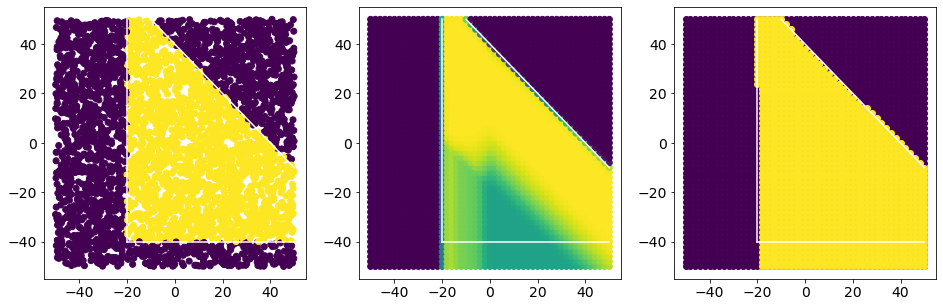
\includegraphics[width=\columnwidth]{Standard_points_0.png}
  \caption{\label{fig:std_dataset_predictions}Training using the reference dataset (3200 + 800 points).}
  \end{subfigure}
  
  \begin{subfigure}{\columnwidth}
  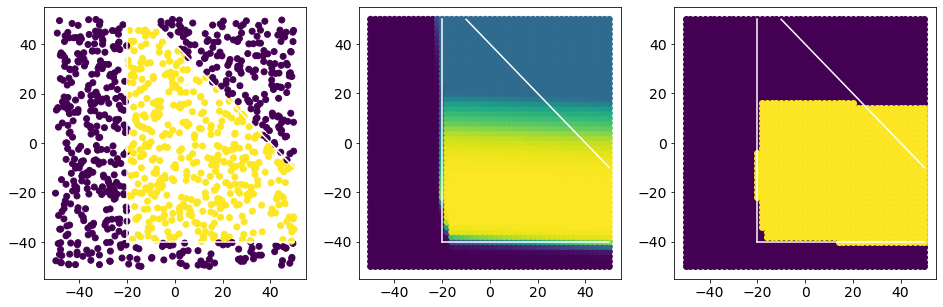
\includegraphics[width=\columnwidth]{Reduced_points_1a.png}
  \caption{\label{fig:reduced_predictions} Training using the reduced dataset (800 + 200 points).}
  \end{subfigure}
  
  \caption{\label{fig:predictions}Prediction grids of the default DNN trained, respectively, on the standard and reduced datasets in 400 epochs.}
\end{figure}




\subsection{The increased dataset}
\label{ssec:increased_dataset}

On the other hand, we can use an increased dataset of $20k$ samples. Considering the $80\%$ splitting, the training set counts $16k$ points, exactly 5 times the reference training dataset size.

In this scenario the model performs better (Figure \ref{fig:increased_predictions}) and the final result is more stable. This result suggests that the size of the dataset is relevant for achieving a good accuracy, at least within the current DNN layout and data pattern. We achieve an accuracy in the order of $\sim 99\%$, while the validation and train loss are comparable (therefore, there are no overfitting issues).

\begin{figure}[h]
  \centering
  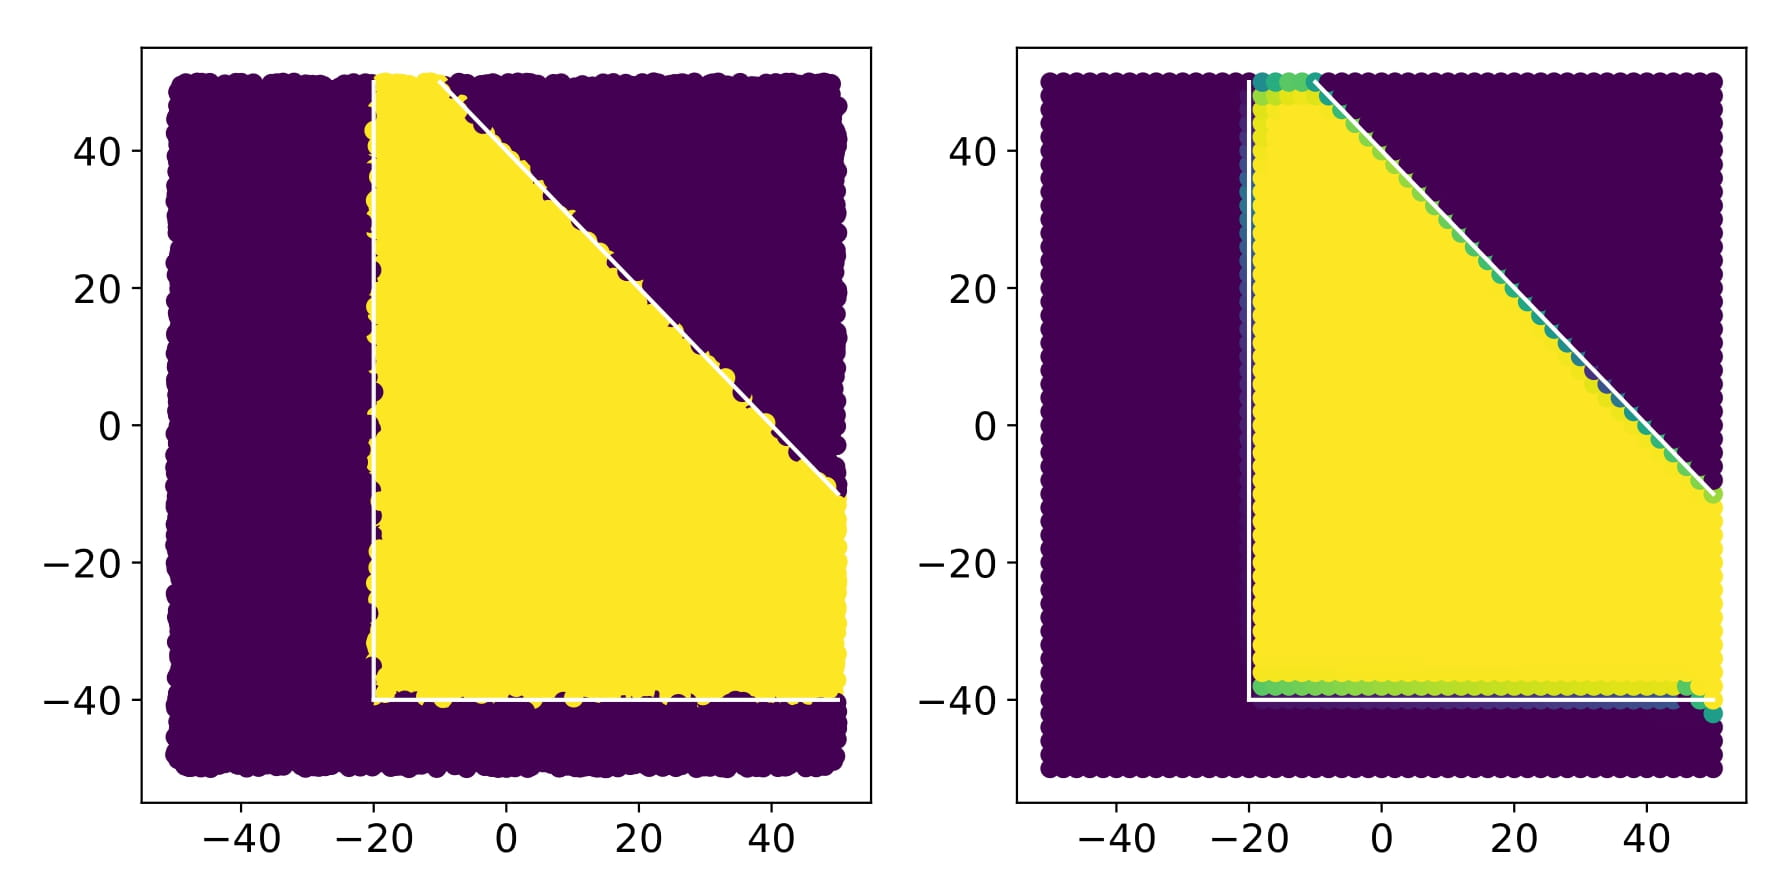
\includegraphics[width=\columnwidth]{dataset_increased_prediction_crop.jpg}
  %\vskip 1mm
  %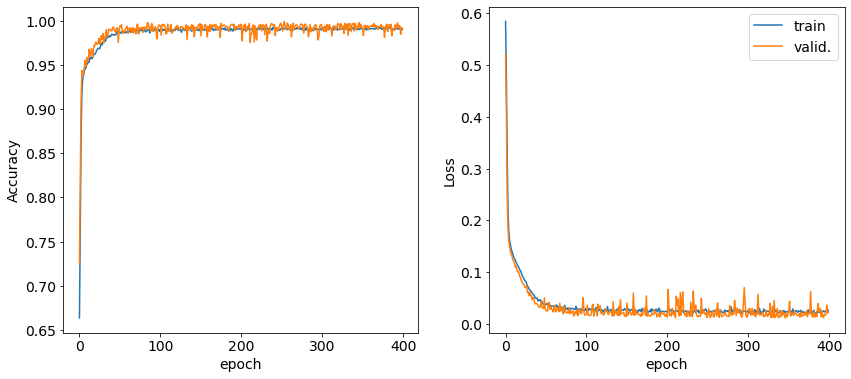
\includegraphics[width=\columnwidth]{Increased_performance_1b.png}
  \caption{On the left, the increased dataset (16k + 4k points). On the right, the prediction grid of the default DNN trained for 400 epochs. }
  \label{fig:increased_predictions}
\end{figure}





\subsection{The augmented dataset}
\label{ssec:augmented_dataset}

The advantages of training with more data samples can also be obtained by applying on the reference dataset a data augmentation technique, which we have implemented from scratch to work on n-dimensional datasets.

%An accuracy similar to the increased dataset's one can be achieved in the case in which the number of samples is artificially increased by applying a data augmentation technique, which we have implemented from scratch.
%There is another way to achieve the same accuracy of the increased dataset: the number of samples can be artificially increased by applying a data augmentation technique, which we have implemented from scratch.

Originally, we performed the data augmentation considering each training sample $(\vec{x},y) = (x_1, x_2, y)$, and generating a fixed number of multiple artificial samples $(\vec{x'}, y)_i = (x_1 + s_1, x_2 + s_2, y)_i$, where $s_1$ and $s_2$ are random displacements drawn from a uniform distribution in $[-\sigma, +\sigma]$. However, we observed that this procedure would have ignored the spatial distribution of the samples' labels. Indeed, there would have been no difference in the displacements for a training sample at the boundary of the triangular region with respect to a sample located far from any boundaries. This would have caused the boundaries to be too shattered. Otherwise, reducing the amplitude of the uniform distribution $\sigma$ would have caused the presence of clusters.

To fix this issue and take into account that our dataset presents boundaries between regions of points, we choose the amplitude of the displacement uniform distribution to vary depending on how close is the point to differently labeled points. %the boundary. %support has the absolute minimum for samples surrounded by fifty-fifty labels, then it grows until it reaches the absolute maximum for samples surrounded by labels all of the same type.

For 2D datasets, the procedure is the following:
\begin{itemize}
    \setlength{\itemsep}{0pt}
    \setlength{\parskip}{0pt}
    \setlength{\parsep}{0pt}
    \item at each iteration, a random sample $C_j$ is drawn from the training dataset
    \item we select all the samples $\vec{x}_i$ enclosed in a rectangle centered on $C_j$ (each side is chosen to be $1/20^{th}$ of the corresponding domain range)
    \item we compute the relative frequency $f_y$ of the most common label among the points $\vec{x}_i$ and we set the amplitude $\sigma$ of the displacement uniform distribution to be $\sigma = 3\cdot(f_y)^3$
    \item each point $\vec{x}_i$ is used to compute an identically labeled artificial sample $\vec{x'}_i = ( x_1 + s_1, x_2 + s_2)_i$ 
\end{itemize}
This procedure is repeated according to a parameter, which we call \emph{augmentation factor} $E$. Eventually, the number of samples is increased approximately to $E$ times the size of the initial dataset.

\begin{table}[h]
\begin{tabular}{ccc}
\hline\hline
Augmentation factor & Train accuracy & Validation accuracy \\ \hline
(no augmentation)   & 0.9278         & 0.9253              \\
2                   & 0.9857         & 0.9306              \\
3                   & 0.9826         & 0.9869              \\
10                  & 0.9749         & 0.9912              \\ 
20                  & 0.9740         & 0.9937              \\ %\hline\hline
30                  & 0.9768         & 0.9962              \\ \hline\hline
\end{tabular}
\caption{\label{tab:augmentation_accuracy}Accuracy of the DNN when different augmented datasets are prompted.} %We notice that the validation accuracy rapidly saturates to $> 99\%$.} 
\end{table}

We observe that a greater set size, even if artificially augmented, leads to a saturation of the model accuracy (Table \ref{tab:augmentation_accuracy}). This is reasonable, as it is not possible to indefinitely draw more and more constructive information from the same sample of training data. Furthermore, the additional samples act as stabilizers when we check the accuracy over independent training iterations.